\section{Rollout Forecasting Results}
To evaluate long-term emulation capability, we performed a complete 142-step (710-day) autoregressive rollout on independent Test Case 5. The models were initialized using the ground-truth state for the first three timesteps (to populate the pressure history lag features) and then run in a fully autonomous rollout mode, feeding their own state predictions back as inputs for subsequent timesteps.

\subsection{Loss-Weight Sweep Configuration Results}
The performance of the three multi-objective loss configurations is evaluated in a hyperparameter sweep over a 20-epoch training span. The pressure-heavy configuration ($0.7\mathcal{L}_P + 0.3\mathcal{L}_{S_g}$) achieves the lowest composite balance score of \textbf{0.00536}, corresponding to a mean pressure RMSE of 22.29~bar and a mean gas saturation RMSE of 0.02407. In contrast, the balanced loss configuration ($0.5\mathcal{L}_P + 0.5\mathcal{L}_{S_g}$) and the saturation-heavy configuration ($0.3\mathcal{L}_P + 0.7\mathcal{L}_{S_g}$) yield higher composite scores of 0.00630 and 0.01209, respectively. 

The sweep establishes the pressure-heavy formulation as the optimal configuration for multi-objective training under our target weighting criteria. The training and validation loss profiles (weighted MSE) for these configurations are plotted in Fig.~\ref{fig:training_curves}, showing stable convergence.

\subsection{Autoregressive Rollout Evaluation}
Using the winning pressure-heavy configuration as the loss function, we compared three versions of the ST-GNN architecture to assess the impact of structural and training enhancements:
\begin{enumerate}
    \item \textbf{ST-GNN v1}: The baseline architecture (hidden dimension $d_h = 64$), trained for 12 epochs under pure teacher forcing.
    \item \textbf{ST-GNN v2}: The enhanced architecture (hidden dimension $d_h = 128$) featuring residual skip connections and LayerNorm, trained for 30 epochs under the scheduled sampling curriculum.
    \item \textbf{ST-GNN v3}: The hyperparameter sweep winner (hidden dimension $d_h = 128$), trained for 60 epochs using the optimal $0.7\mathcal{L}_P + 0.3\mathcal{L}_{S_g}$ loss weighting.
\end{enumerate}

The stepwise autoregressive rollout RMSE values for pressure and gas saturation are summarized in Table~\ref{tab:rollout_metrics}, and their temporal evolution is plotted in Fig.~\ref{fig:rollout_rmse}.

Quantitatively, the ST-GNN v2 model yields a \textbf{31.63\% reduction} in final-step pressure RMSE compared to v1 (33.67~bar vs. 49.25~bar) and a \textbf{10.04\% reduction} in mean pressure RMSE over the entire rollout (31.72~bar vs. 35.26~bar). These improvements suggest that incorporating LayerNorm and residual skip connections stabilizes training gradients in deeper graph structures, while scheduled sampling mitigates covariate shift during autoregressive rollouts.

However, long-horizon error accumulation remains a major challenge. The pressure RMSE in ST-GNN v2 increases from 0.19~bar at step 1 to 1.83~bar at step 10, and reaches a peak of 59.19~bar at step 50 before partially recovering and equilibrating to 33.67~bar at the final step (step 146). The peak error near step 50 coincides with the transition from the injection phase to the shut-in phase, where the reservoir undergoes rapid pressure redistribution that the model struggles to track. 

To visualize rollout quality, Fig.~\ref{fig:pressure_tracking} and Fig.~\ref{fig:saturation_tracking} compare the simulator ground truth and the GNN predictions for pressure and gas saturation at representative locations in the reservoir. A summary of discrete rollout step error benchmarks is illustrated in Fig.~\ref{fig:bar_comparison}.

\begin{table*}[t]
\centering
\caption{ST-GNN Rollout Metric Comparison (Averaged Over 142 Steps)}
\label{tab:stgnn_comparison}
\begin{tabular}{lcccc}
\toprule
\textbf{Model} & \textbf{Mean $P$-RMSE (bar)} & \textbf{Mean $S_g$-RMSE} & \textbf{Max $P$-Error (bar)} & \textbf{Max $S_g$-Error} \\
\midrule
\textbf{ST-GNN v1} & 35.2638 & 0.016717 & 278.29 & 0.3960 \\
\textbf{ST-GNN v2} & 31.7239 & 0.022283 & 240.64 & 0.4041 \\
\textbf{ST-GNN v3 (sweep)} & \textbf{27.1501} & 0.018108 & \textbf{187.68} & 0.4258 \\
\bottomrule
\end{tabular}
\end{table*}

\begin{table}[h]
\centering
\caption{Multi-Step Autoregressive Rollout RMSE Details on Test Case 5}
\label{tab:rollout_metrics}
\begin{tabular}{lcccc}
\toprule
\textbf{Model \& State Variable} & \textbf{t = 1 step} & \textbf{t = 10 steps} & \textbf{t = 50 steps} & \textbf{t = 146 steps (Final)} \\
\midrule
\textbf{Pressure RMSE (bar)} \\
ST-GNN v1 (12 epochs) & 0.3568 & 4.5491 & 75.5759 & 49.2455 \\
ST-GNN v2 (30 epochs) & 0.1900 & \textbf{1.8337} & \textbf{59.1941} & 33.6702 \\
ST-GNN v3 (60-ep sweep winner) & \textbf{0.1008} & 2.2427 & 72.4473 & \textbf{31.6625} \\
\midrule
\textbf{Saturation RMSE ($S_g$)} \\
ST-GNN v1 (12 epochs) & 0.003025 & 0.012442 & \textbf{0.025100} & \textbf{0.016476} \\
ST-GNN v2 (30 epochs) & 0.001621 & 0.006212 & 0.030784 & 0.029837 \\
ST-GNN v3 (60-ep sweep winner) & \textbf{0.000922} & \textbf{0.003486} & 0.028324 & 0.029365 \\
\bottomrule
\end{tabular}
\end{table}

\subsection{Model Selection: ST-GNN v2 versus ST-GNN v3}
To determine the preferred configuration for future investigation within the current proof-of-concept framework, we perform a quantitative trade-off analysis between ST-GNN v2 and ST-GNN v3. The two architectures optimize different facets of the autoregressive forecasting rollout. Under ST-GNN v3, the hyperparameters were tuned via a multi-objective sweep that selected the pressure-heavy loss configuration ($0.7\mathcal{L}_P + 0.3\mathcal{L}_{S_g}$), which after 60 epochs of training achieves a mean pressure RMSE of 27.15~bar (representing a 14.4\% reduction from v2's mean pressure RMSE of 31.72~bar) and a mean gas saturation RMSE of 0.01811 (a 18.7\% reduction from v2's mean saturation RMSE of 0.02228). 

Furthermore, ST-GNN v3 demonstrates superior stability at the end of the rollout, with its final-step pressure RMSE bounded at 31.66~bar. This represents a 6.0\% reduction in final-step pressure error compared to v2 (33.67~bar) and a 32.5\% reduction in maximum pressure error (187.68~bar vs. 240.64~bar). This improvement is attributed to the extended training duration (60 epochs), which allowed the scheduled sampling curriculum to successfully bridge the transition from teacher forcing to fully autoregressive feedback. Consequently, ST-GNN v3 is selected as the preferred configuration for future investigation within the current proof-of-concept framework and preliminary screening.

\subsection{Model Variability and Reproducibility}
\label{subsec:uq}
Due to computational constraints, the ST-GNN models presented in this work were trained using a single random seed for weight initialization and training batch permutations. Consequently, the reported RMSE metrics and rollout profiles do not represent statistical averages across multiple trials and lack confidence intervals. In deep learning surrogates, model variability can arise from stochastic weight initialization and training batch ordering, which may affect the specific timestep at which error accumulation accelerates during rollout. A rigorous uncertainty quantification study would require training an ensemble of models (e.g., $N=10$ runs with different seeds) to compute the mean and standard deviation of rollout errors over time. We identify this ensemble-based uncertainty quantification as a critical area for future work, which will provide bounds on surrogate prediction confidence for risk-managed reservoir operations.

\begin{figure}[htbp]
    \centering
    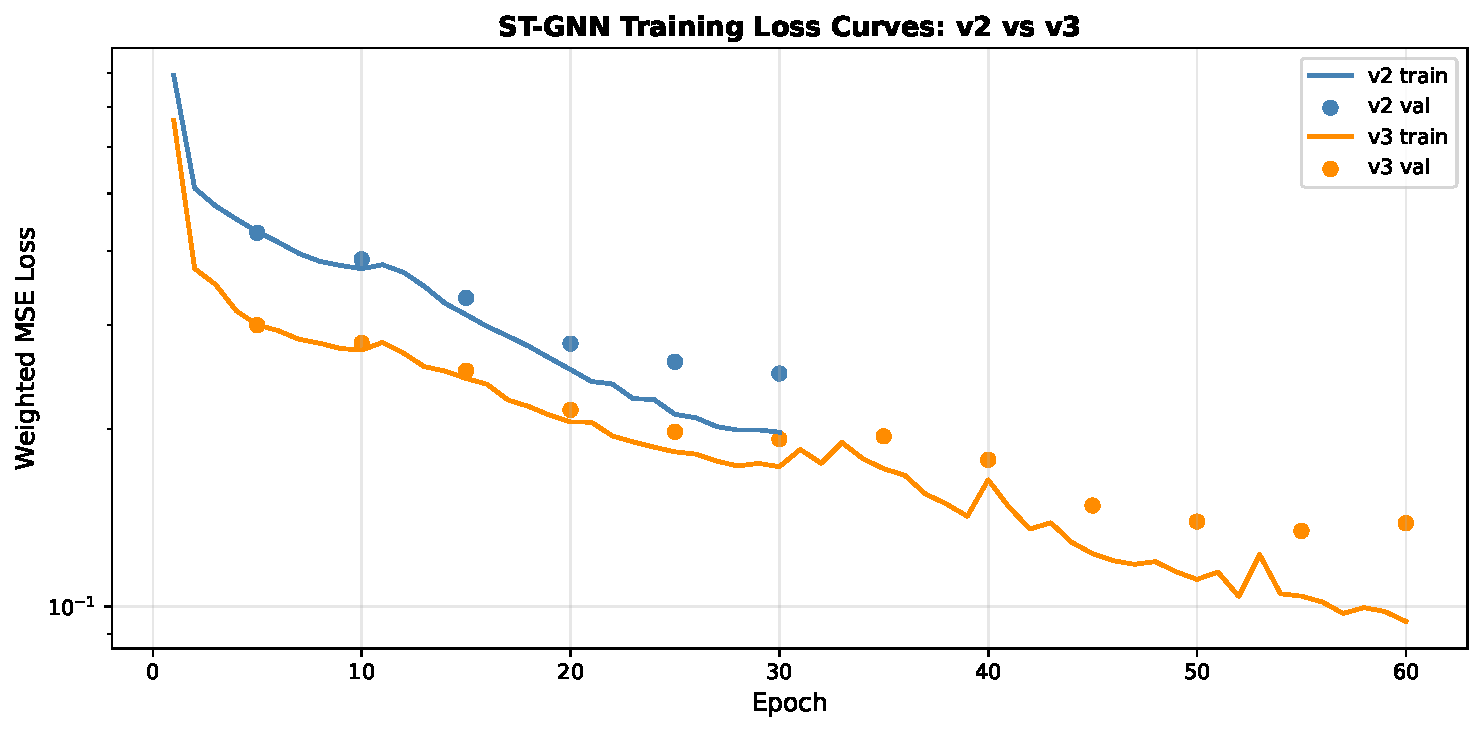
\includegraphics[width=0.95\columnwidth]{figures/fig8_training_curves}
    \caption{Training and validation loss curves (weighted MSE) over epochs for the ST-GNN configurations, showing stable convergence profiles.}
    \label{fig:training_curves}
\end{figure}

\begin{figure}[htbp]
    \centering
    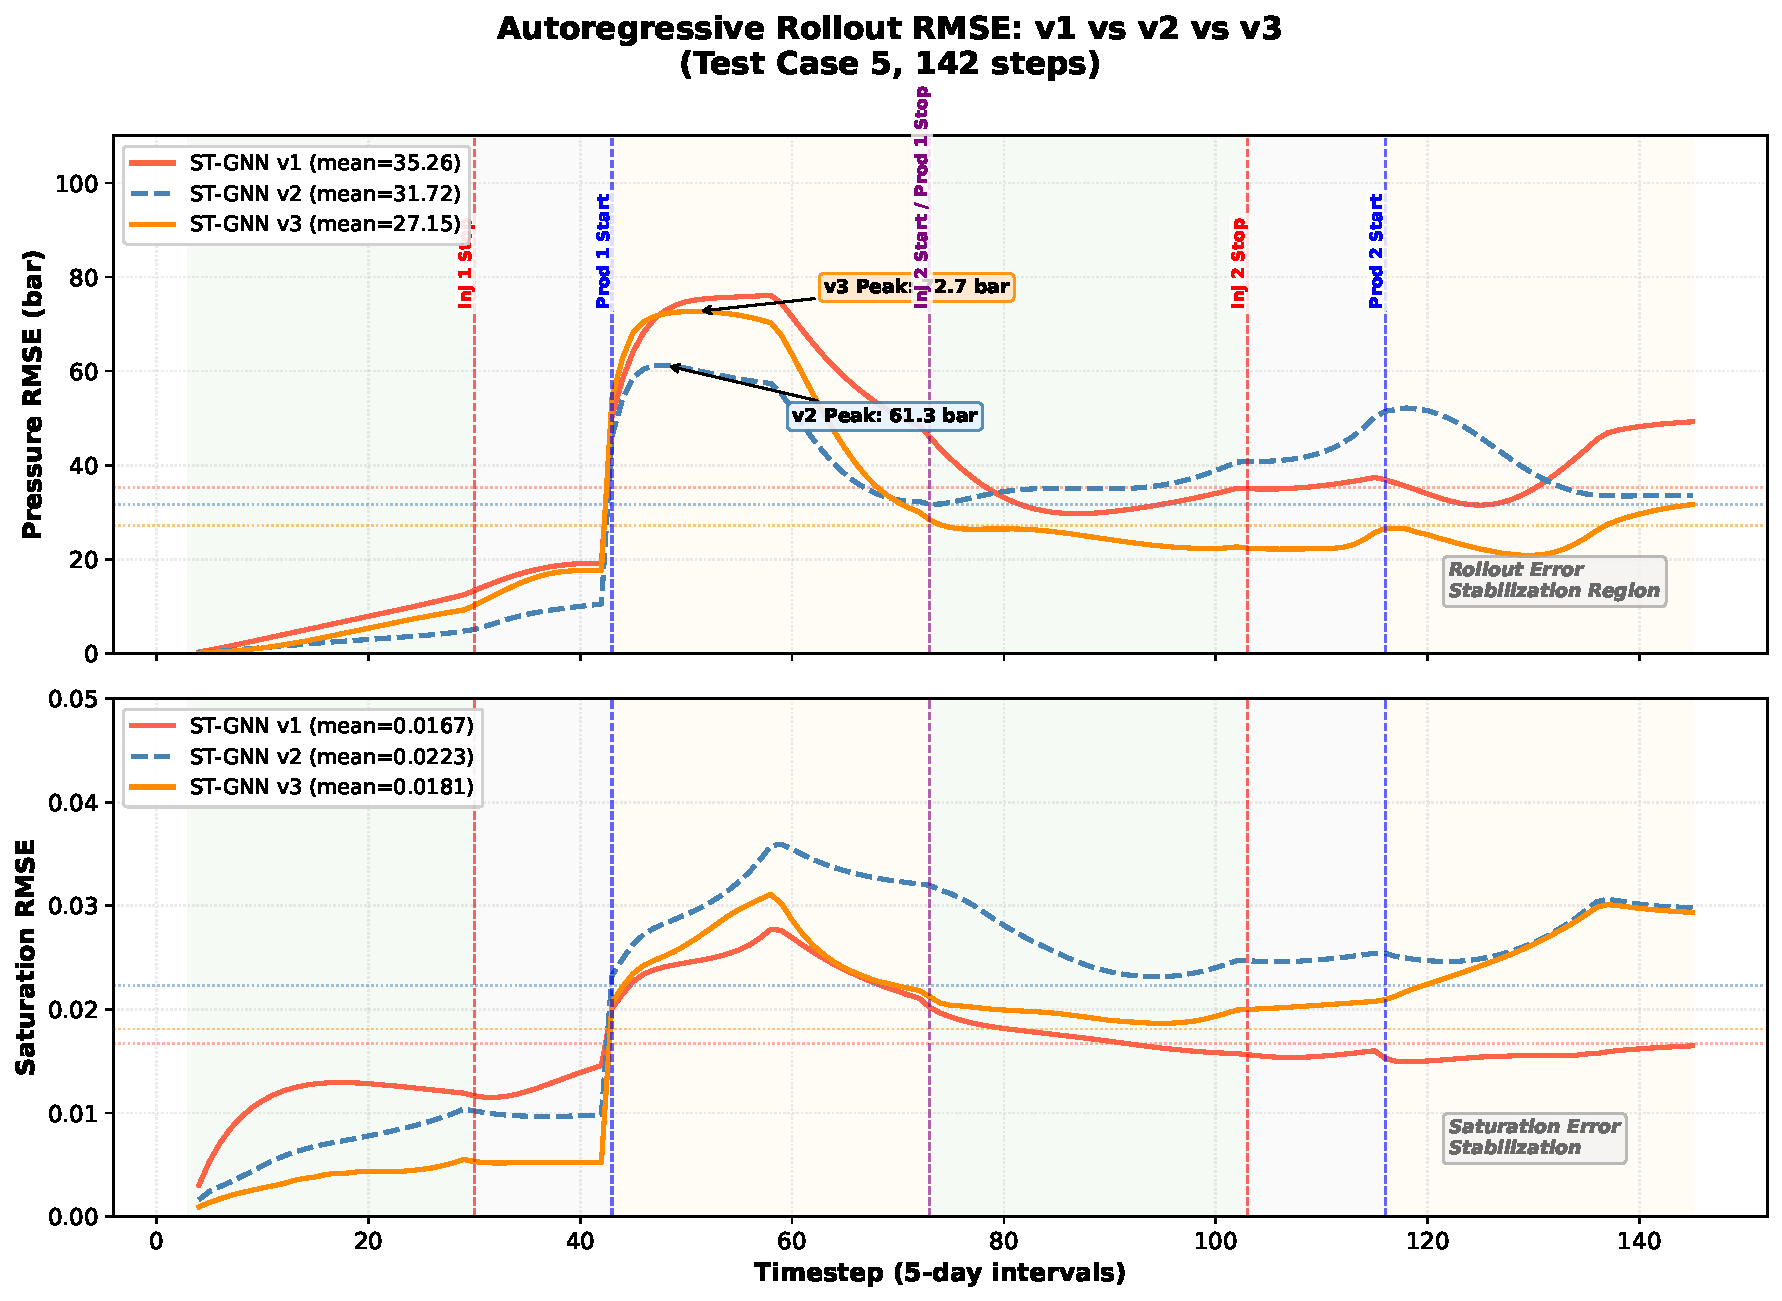
\includegraphics[width=0.95\columnwidth]{figures/fig9_rollout_rmse}
    \caption{Autoregressive rollout RMSE over the 142-step forecasting horizon on Test Case 5. Left: Pressure RMSE (bar). Right: Gas saturation ($S_g$) RMSE.}
    \label{fig:rollout_rmse}
\end{figure}

\begin{figure*}[t]
    \centering
    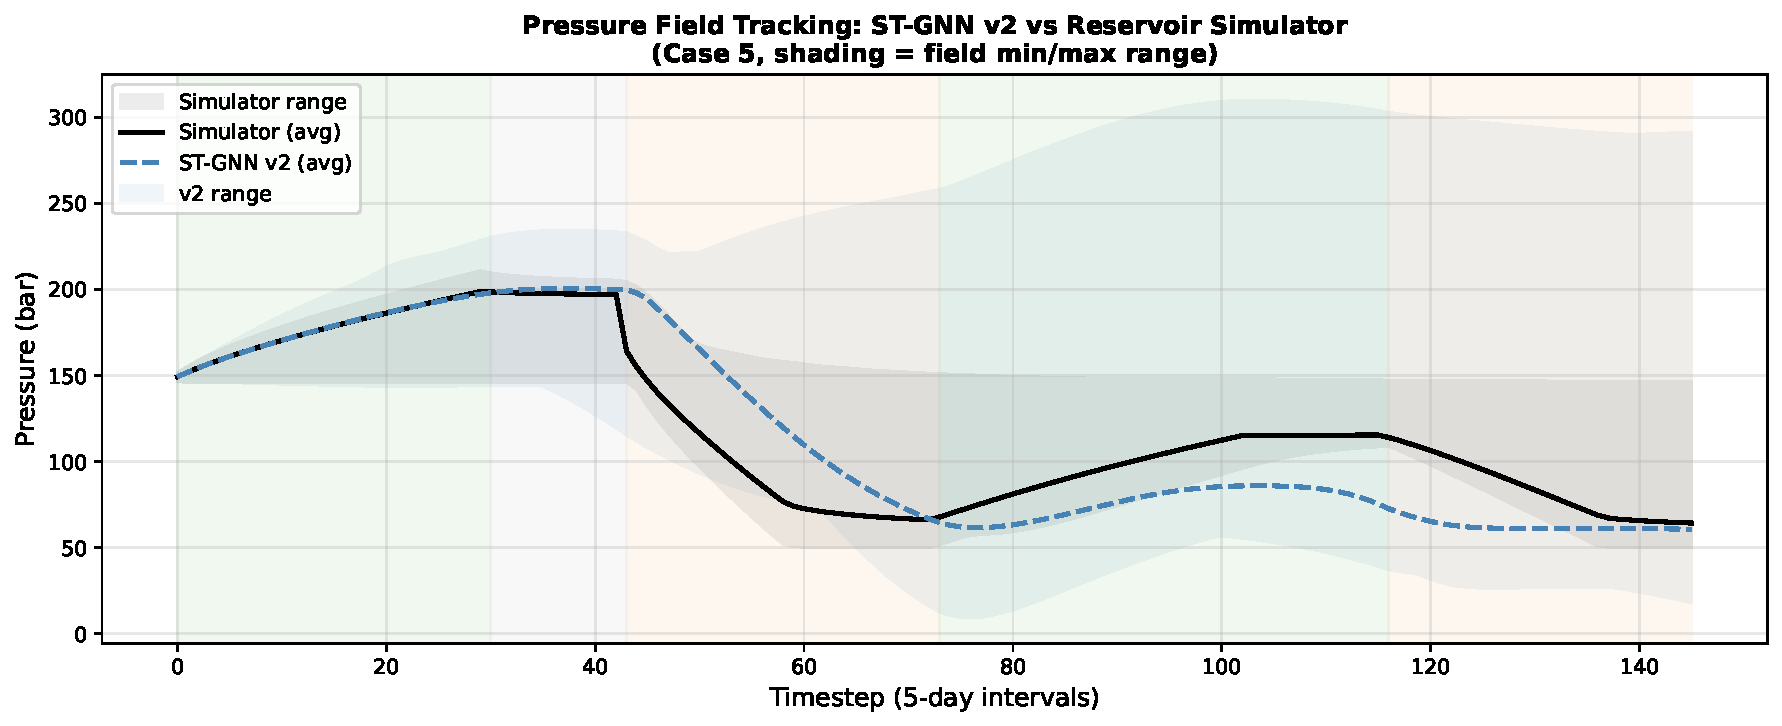
\includegraphics[width=\textwidth]{figures/fig10_pressure_tracking}
    \caption{Pressure tracking comparisons between numerical reservoir simulator ground truth (solid lines) and ST-GNN v2 predictions (dashed lines) at select grid locations over the rollout.}
    \label{fig:pressure_tracking}
\end{figure*}

\begin{figure*}[t]
    \centering
    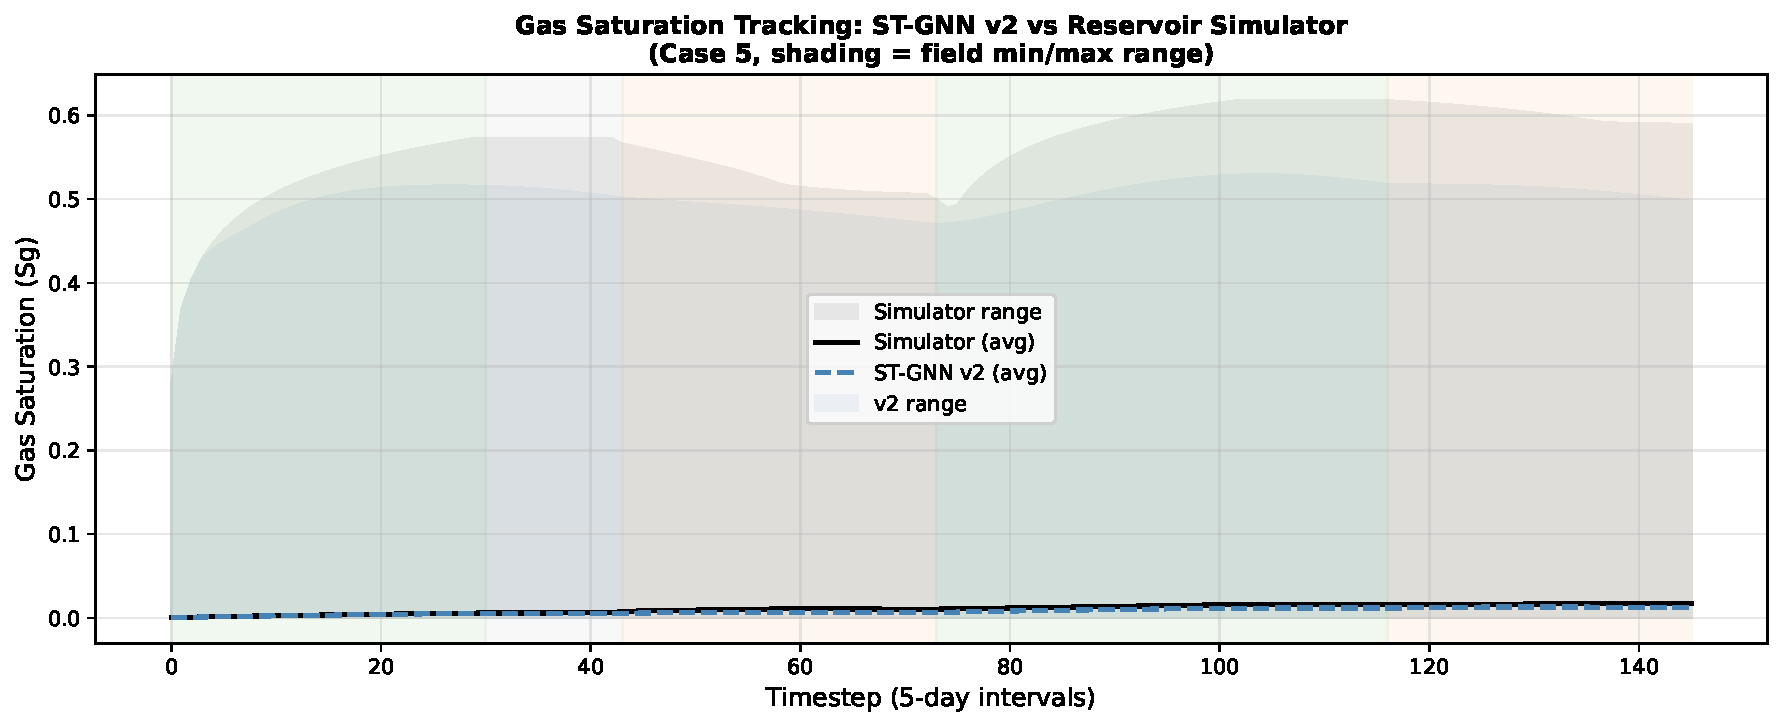
\includegraphics[width=\textwidth]{figures/fig11_saturation_tracking}
    \caption{Gas saturation ($S_g$) tracking comparisons between numerical reservoir simulator ground truth (solid lines) and ST-GNN v2 predictions (dashed lines) at select grid locations over the rollout.}
    \label{fig:saturation_tracking}
\end{figure*}

\begin{figure*}[t]
    \centering
    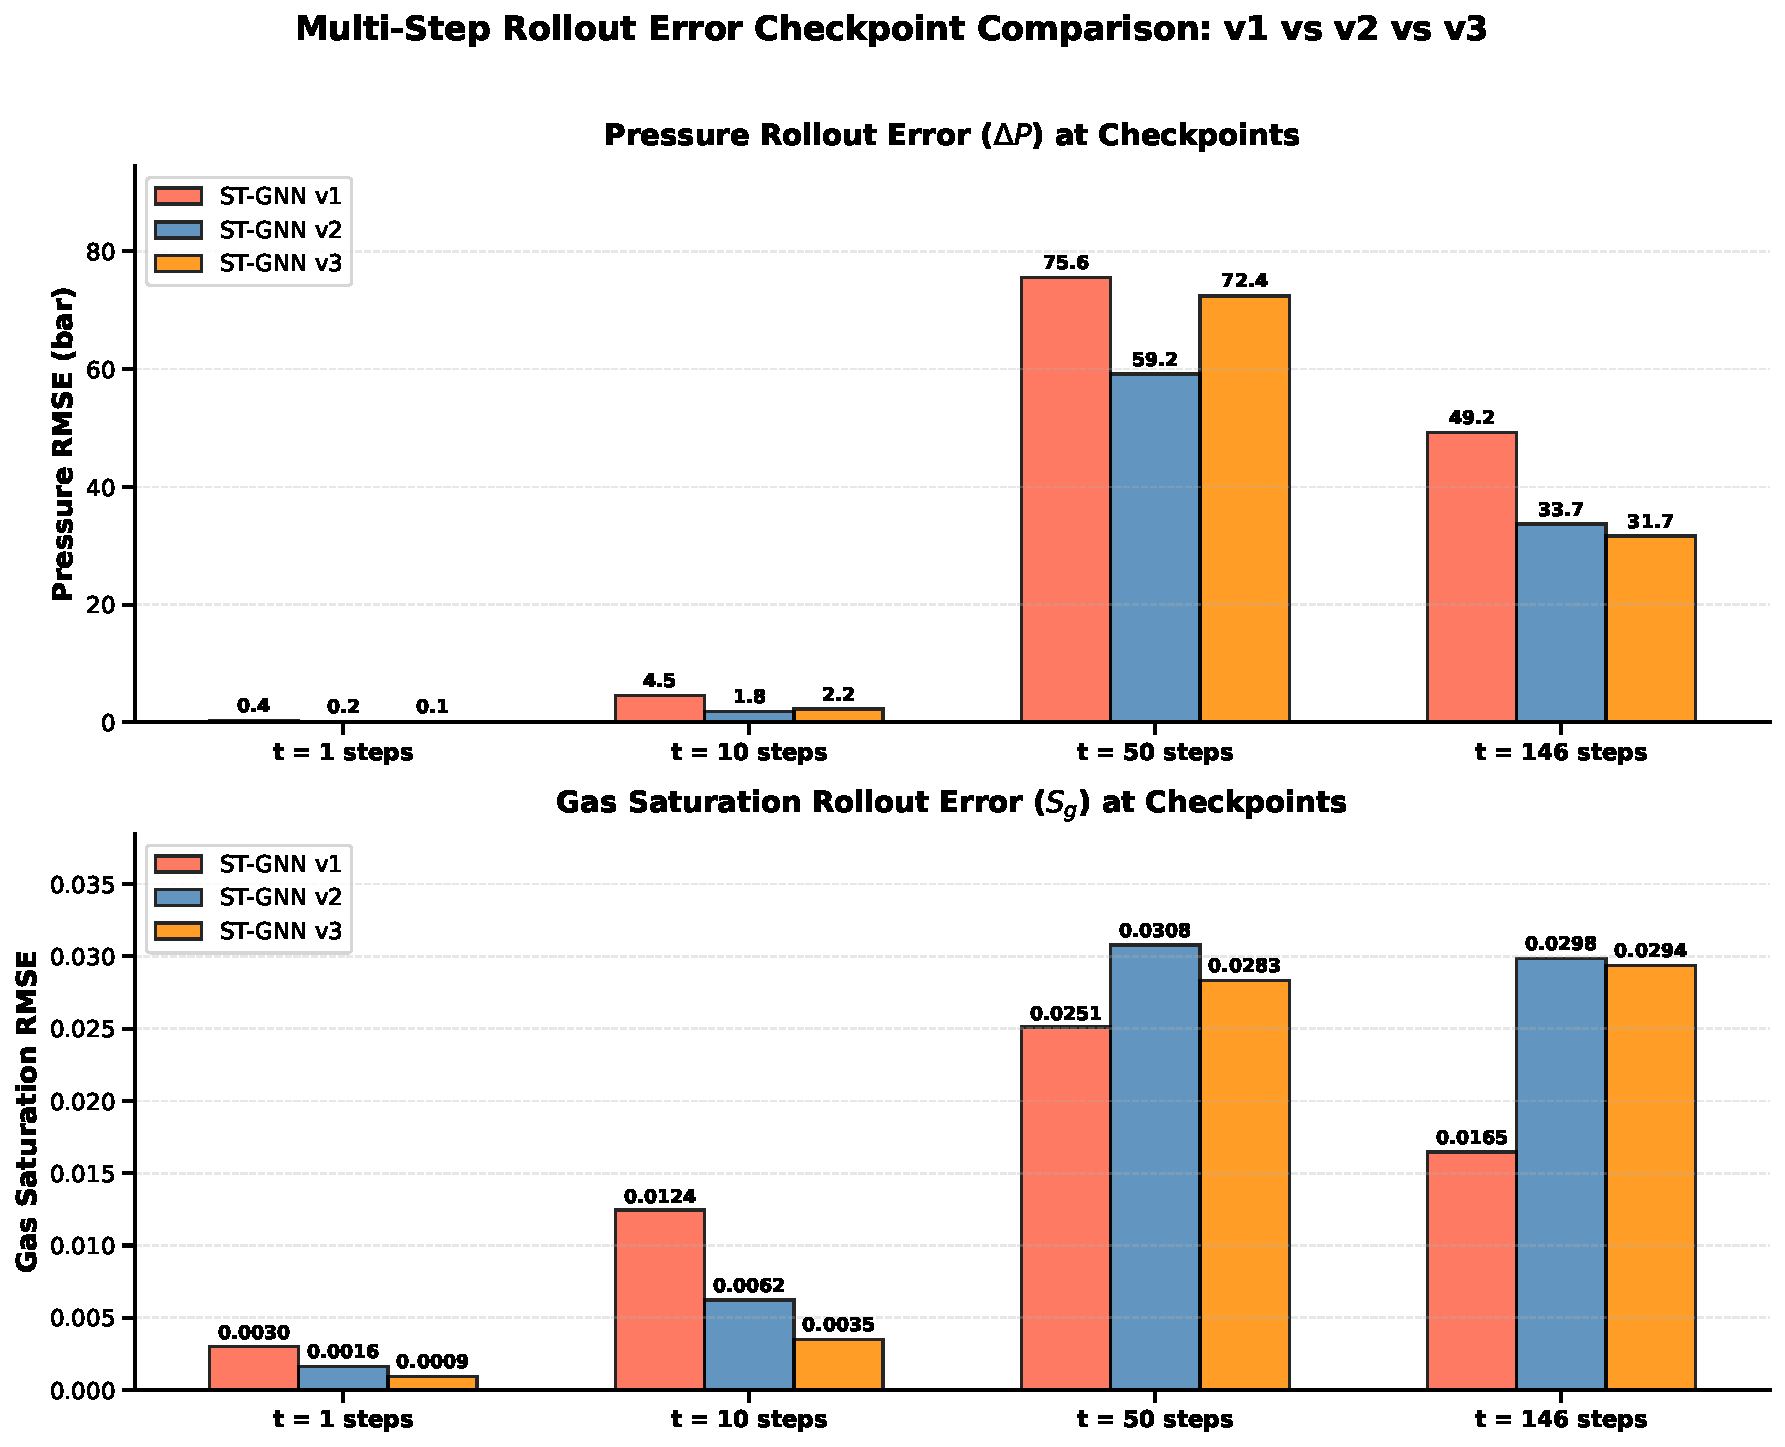
\includegraphics[width=\textwidth]{figures/fig12_bar_comparison}
    \caption{Multi-step rollout comparison bar charts showing pressure and saturation errors at discrete rollout steps (t = 1, 10, 50, and 146) for ST-GNN v1, v2, and v3.}
    \label{fig:bar_comparison}
\end{figure*}
